\documentclass[english]{article}

\usepackage[latin9]{inputenc}
\usepackage[letterpaper]{geometry}
\geometry{verbose,tmargin=1in,bmargin=1in,lmargin=1in,rmargin=1in}
\usepackage{amsmath}
\usepackage{amssymb}
\usepackage{graphicx}

\title{CIS 581, Computer Vision, Fall 2015: Project3 \\
Yu-Cheng Lin}
\date{}

\begin{document}
\maketitle
\section*{Introduction}
This document provides a brief explanation of the more notable parts of my implementation of project3. This report is written under the assumption that the reader already has a very good understanding of all the steps of the project.
\section*{Seam Carving}
As far as seam carving goes, we use djikstra's algorithm to find the path of least cost. In this particular implementation, the cost is defined by the "edgeness" of a pixel (length of the gradient vector). A seam with the least cumulative "edgeness" is removed upon each iteration. As long as I don't remove too many seams, the image would look reasonable.
\\\\
Let's look at an uncarved image of spicy hotpot\\\\
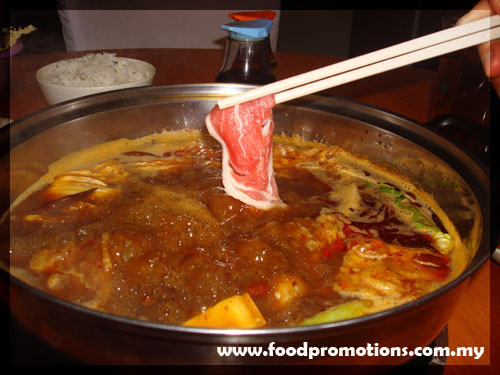
\includegraphics[scale=0.8]{carving/hotpot.jpg}\\
This image is a good example because this image breaks the algorithm early, but I still have a high probability of successfully removing a seam that does not cause much difference visually. Let's check out the image with 100 columns of pixels removed\\\\
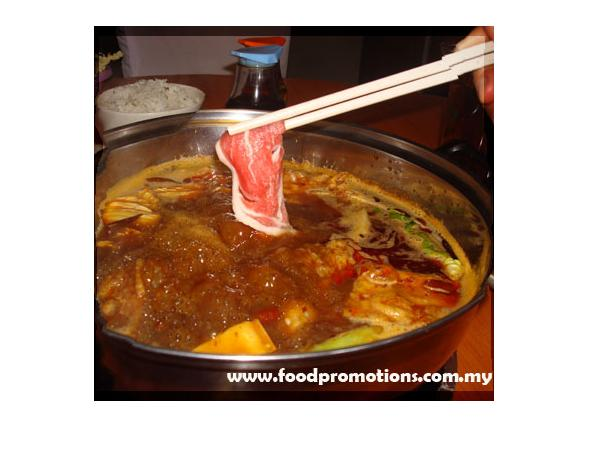
\includegraphics[scale=0.8]{carving/hotpot100removed.jpg}\\
We can see the rim of the pot gets warped and the chopstick gets distorted. This happens because I have very strong edges across the horizontal direction that I even eventually have to remove some of them. However, the contents of the pot look fine. Even though there are some strong edges being removed, my brain registers the content of the pot as a testure. Therefore I think the content is fine. Let's look at the image with 200 columns removed\\\\
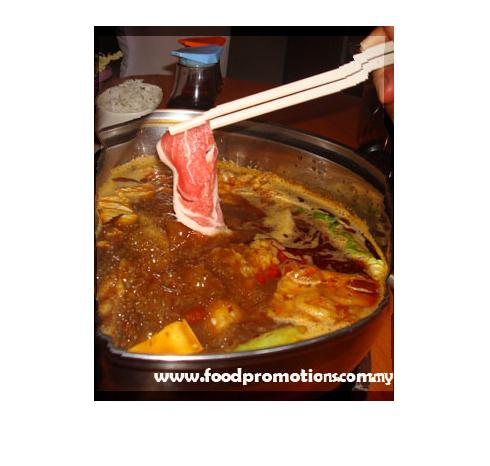
\includegraphics[scale=0.8]{carving/hotpot200removed.jpg}\\
The warping gets a little worse, but most of the visual cues still stays in tact.\\\\
Now Let's look at some other cool examples\\\\
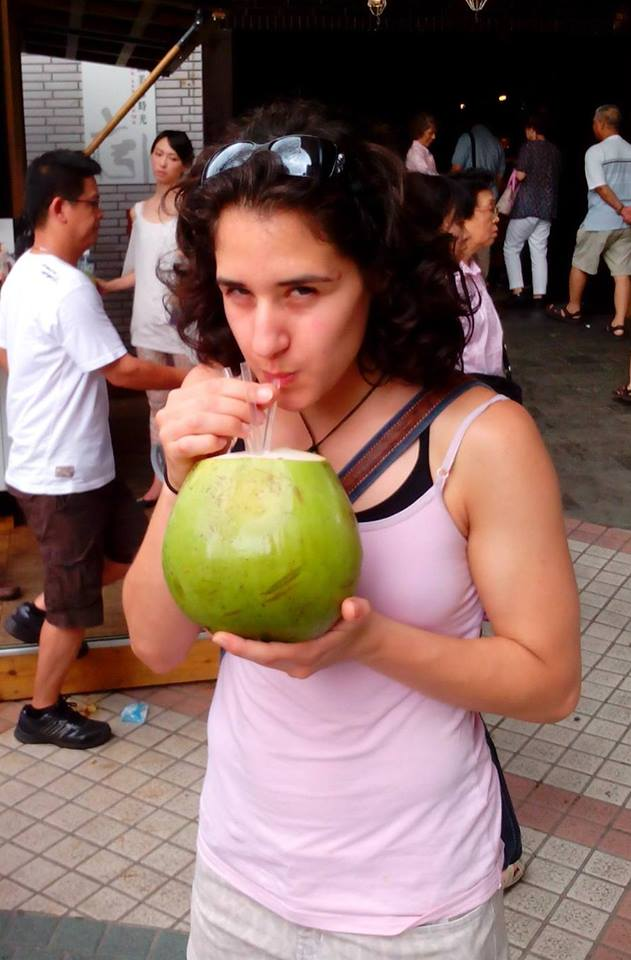
\includegraphics[scale=0.6]{carving/lola.jpg}\\\\
let's carve 50 columns\\\\
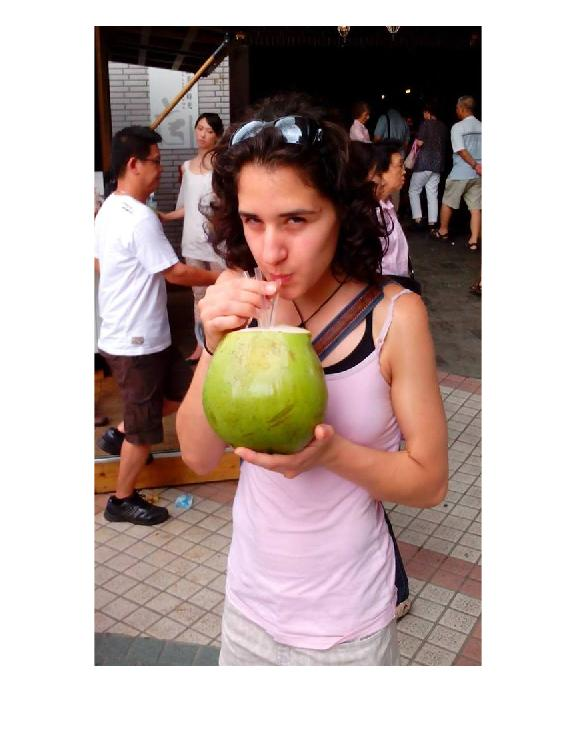
\includegraphics[scale=0.6]{carving/lola100removed.jpg}\\\\
The algorithm avoided the tiles on the floor because there are very strong edges. So the algorithm resorted to carving the girl's body. Interestingly, the face stays in tact. This image looks a little odd, but still reasonable to the human eye.

\section*{Optimal Seam Carving}

So now the grand question, if I need to remove a set number of rows and columns, what is the optimal sequence to remove them. First, we know that a naive search should be out of question since it takes $O(C^N)$ time to search, plus image processing in the innerloop. We will resort to a slightly greedy djikstra's as shown in the paper. The result looks reasonable. \\
removing 50 rows and columns of the hotpot image.\\\\
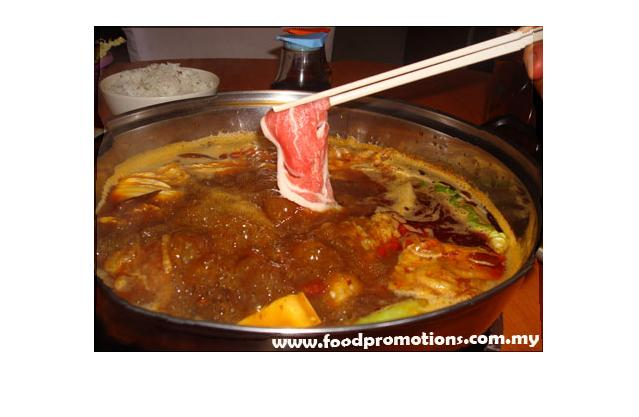
\includegraphics[scale=0.8]{carving/hotpot5050.jpg}\\\\
This method still take a while to compute, but we are able to carve the image within the human patience limit in 2015.

\section*{Image mosaicing}
I hand rolled all the methods in this part of the project, mostly by following the instructions of the project handout. Here are the more notable things in my implemetnation. 
\begin{itemize}
\item {\bf Threshold first in adaptive non-maximum supression}\\
Thresholding first greatly improves the running time of the project. It also makes sense to threshold first since we don't need that many corners. Basically points with small cornerness should be supressed regardless of whether it's a local maxima or not
\item{\bf In feature matching, take a threshold of $<0.1$ to improve performance}\\
We only need 4 correspondences to establish a homography. It is not very costly to get rid of most corners. In fact, it is beneficial to cut out the bad corners to ensure the quality of the transformation.
\item{\bf Debugging method}\\
Visual debugging is the best!\\\\
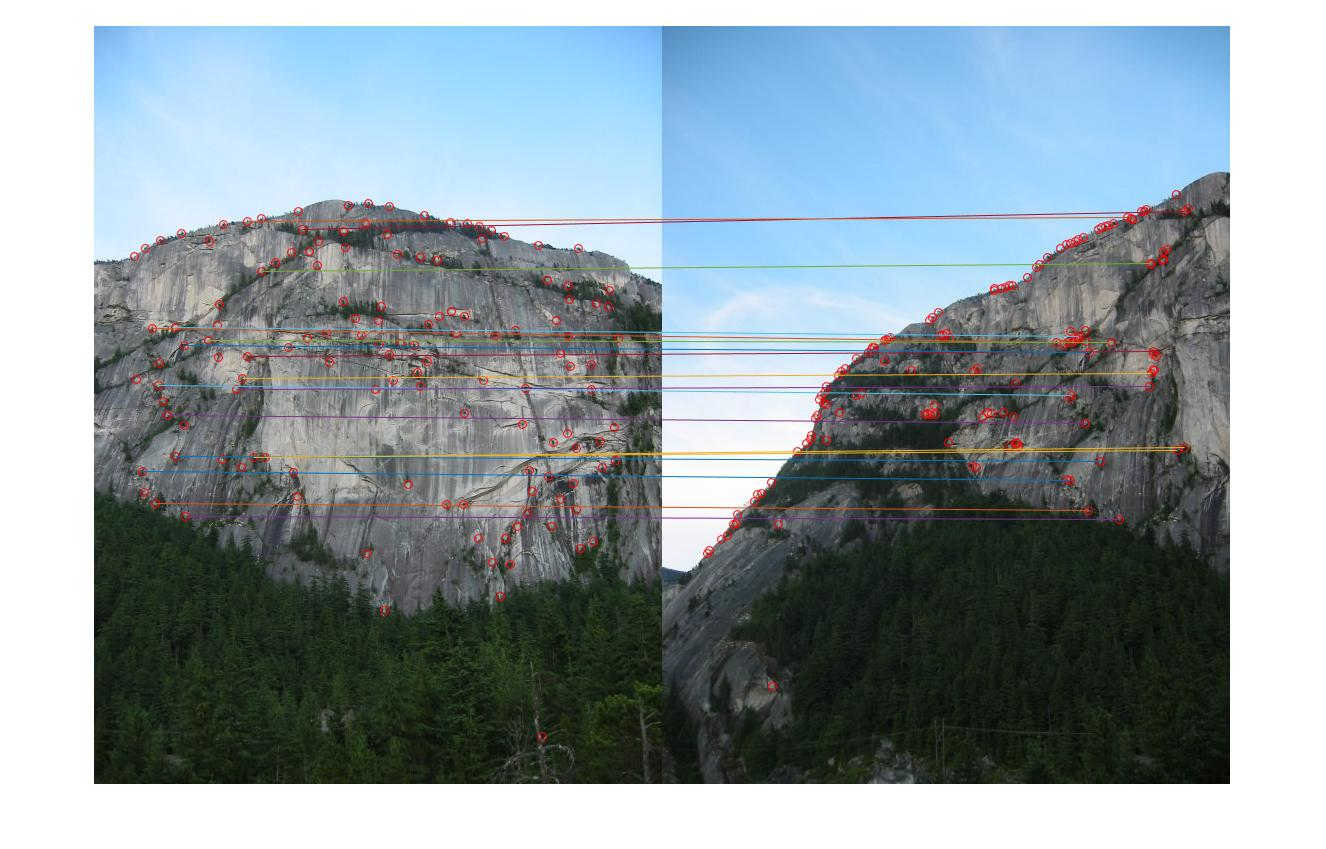
\includegraphics[scale=0.3]{mosaic/mountaindebug.jpg}

\item{\bf Actual stitching}
Used alpha blending, the image does not have visible seam due to different illumination.

\end{itemize}

\section*{Mosaicing results}
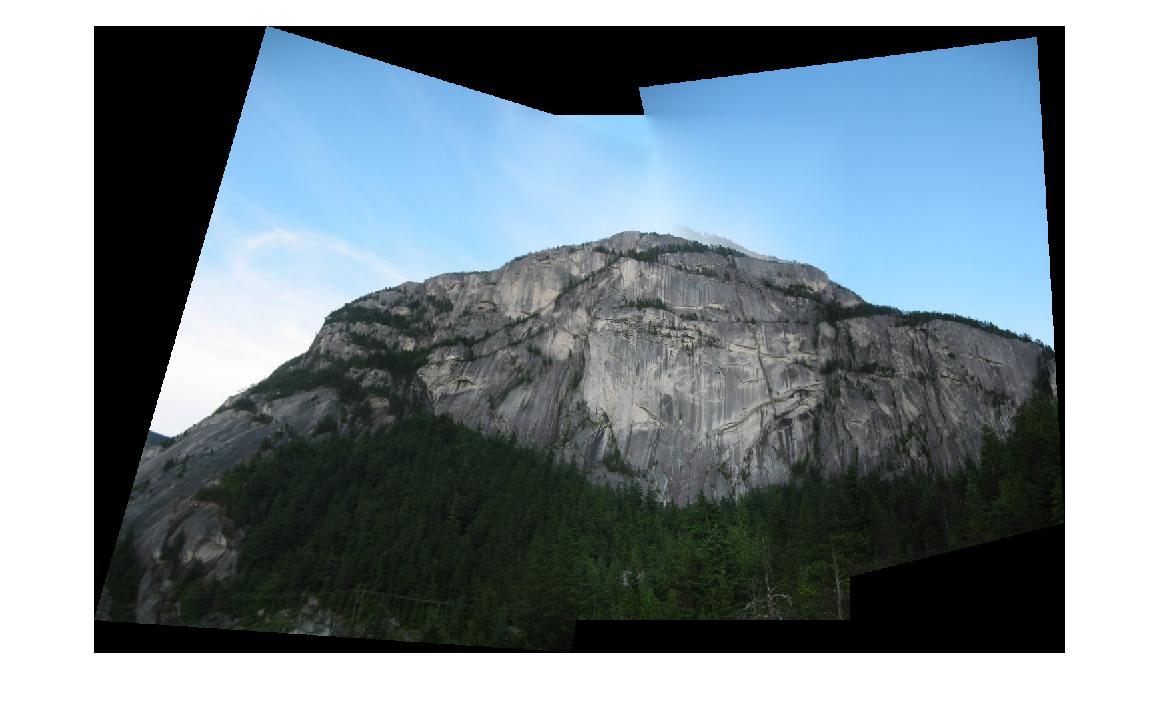
\includegraphics[scale=0.5]{mosaic/mountain.jpg}\\\\
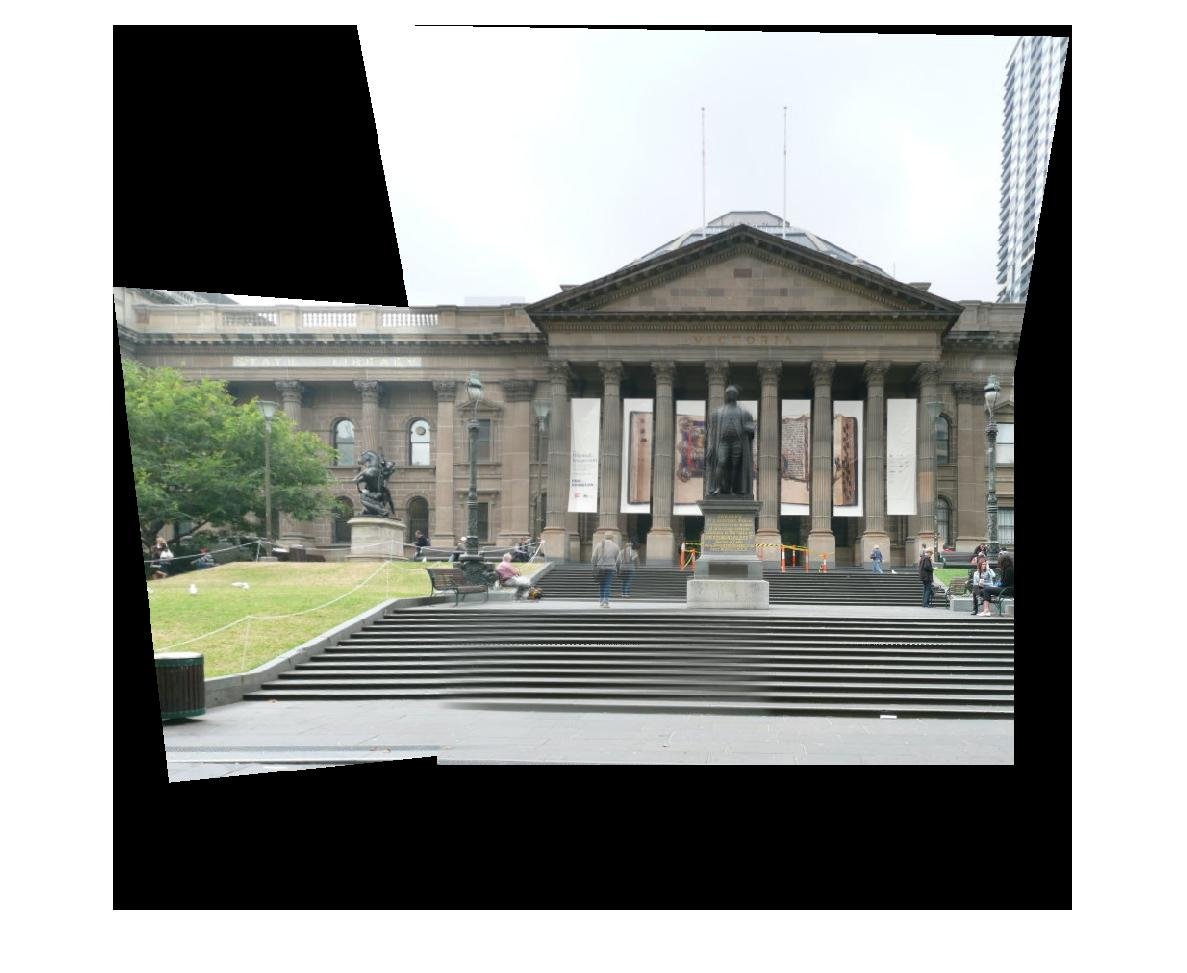
\includegraphics[scale=0.5]{mosaic/rockey.jpg}\\\\
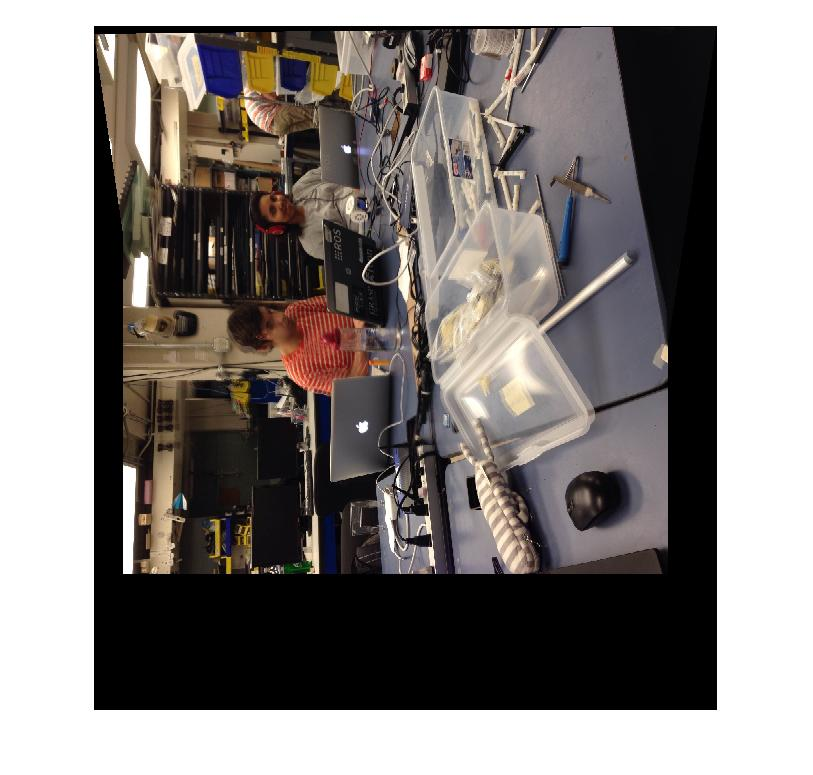
\includegraphics[scale=0.7]{mosaic/modlab.jpg}\\\\
note that in the modlab image, Tarik moved his head so now his face becomes ghost.

\end{document}